\documentclass[conference]{IEEEtran}
\IEEEoverridecommandlockouts
% The preceding line is only needed to identify funding in the first footnote. If that is unneeded, please comment it out.
\usepackage{cite}
\usepackage{amsmath,amssymb,amsfonts}
\usepackage{algorithm}
\usepackage{algorithmic}
\usepackage{graphicx}
\usepackage{textcomp}
\usepackage{xcolor}
\usepackage{bm}
\def\BibTeX{{\rm B\kern-.05em{\sc i\kern-.025em b}\kern-.08em
    T\kern-.1667em\lower.7ex\hbox{E}\kern-.125emX}}
\begin{document}

\title{Orientation Tracking with Neural Network}

\author{\IEEEauthorblockN{Muhammad Fadli Alim Arsani}
\IEEEauthorblockA{\textit{Electrical \& Computer Engineering (ECE) Dept.} \\
\textit{University of California San Diego}\\
San Diego, United States \\
fadlialim0029@gmail.com}
}

\maketitle

\begin{abstract}
The quest for precise 3D orientation tracking of rotating bodies underpins advancements in robotics, augmented reality, and navigational systems, necessitating methodologies that balance accuracy with computational feasibility. This paper uses a Neural Network methodology, innovatively applied to orientation estimation through sensor fusion from a 6-DOF inertial measurement unit (IMU). As for the ground truth data, we use orientation predictions from a VICON motion capture system.

Our investigation reveals the Neural Network accuracy is good for estimating pitch and roll angles but fails to learn discontinuities in the yaw angles. The practical utility of these orientation estimation methods can be demonstrated through the application of panoramic image stitching.

This study underscores Neural Network's potential as a robust alternative for 3D orientation tracking if given more datasets to train on, offering insights into its comparative performance against traditional EKFs. By investigating the strengths and limitations of this Neural Network approach, this work contributes to the broader discourse on advancing sensor-based orientation estimation, encouraging future efforts to optimize this approach for real-time applications.
\end{abstract}

\begin{IEEEkeywords}
3D Orientation Tracking, Deep Learning, Extended Kalman Filter (EKF), Inertial Measurement Unit (IMU), Sensor Fusion, Quaternion Rotation, Neural Network
\end{IEEEkeywords}

\section{Introduction}
In various fields such as robotics, virtual reality, and navigation, accurately tracking the 3D orientation of rotating bodies is crucial. This capability enhances device interaction with their environment, supporting advanced functionalities. The challenge lies in achieving precise orientation tracking amid sensor noise, dynamic changes, and the need for real-time processing.

Kalman Filter variants (EKF, UKF, etc.) are traditionally favored for this task due to their efficacy with nonlinear
systems and sensor data fusion. However, they require careful noise covariance tuning and can be sensitive to initial conditions, making them less flexible across different scenarios.

Neural Networks offers a promising alternative. By optimizing a cost function related to sensor
measurements, it aims for robust orientation estimates. Its main limitation is the reliance on future data, which
complicates real-time application but could potentially enhance accuracy and robustness compared to kalman filters.

The relevance of improving 3D orientation tracking extends beyond theoretical interest. In practice, better algorithms mean improved system performance in robotics, more immersive experiences in augmented reality, and safer, more reliable navigation when GPS is unavailable.

This paper presents an analysis of this Deep-Learning-based approach using ground truth from a VICON system. We aim to highlight its benefits and limitations relative to EKF, providing insights for future research and application in sensor-based orientation estimation tasks.

\section{Problem Formulation}

The objective of this work is to formulate and solve the problem of estimating the 3D orientation of a rotating body
over time. Let us denote the true orientation of the body at discrete time steps \( t = 1, 2, \ldots, T \) by a sequence
of rotation matrices \( \{\bm{R}_t\}_{t=1}^T \). These true orientations are unknown and are to be estimated from the inertial measurement unit (IMU) data.

The IMU provides angular velocity \( \bm{\omega}_t \in \mathbb{R}^3 \) and linear acceleration \( \bm{a}_t \in \mathbb{R}^3 \)
measurements in the body frame at each time step. The problem is compounded by the presence of noise and potential
biases in the IMU data. The estimated orientations, represented by quaternions \( \{\bm{q}_t\}_{t=0}^T \) with \( \bm{q}
_t \in \mathbb{H} \), the space of unit quaternions, are computed such that they best explain the observed IMU data
under the motion and observation models defined in \ref{eq:motion_model} and \ref{eq:observation_model}.

Thus, let us define the following minimization problem:

\begin{equation}\label{eq:minimization_problem}
\min_{\{\bm{q}_t\}_{t=0}^T} \sum_{t=1}^T \left\| \bm{q}_t - \bm{q}_t^* \right\|^2
\end{equation}
where \( \bm{q}_t^* \) is the true orientation at time \( t \).

We seek to solve this minimization problem using the Neural Network, i.e: find $\bm{q}_{0:T}$ that would minimize the
cost in (1). The motion and observation models, as well as the cost function to be minimized, will be introduced in the following section.

\section{Technical Approach}

The following section will present the technical approach used in this work. The detailed
derivations and explanations of the equations can be found in most literature and papers referenced in the references
section.

\subsection{Data Acquisition \& Augmentation}
In the aim to develop robust orientation tracking systems, the acquisition and preprocessing of data play crucial roles. Our study leverages data obtained from a graduate-level course lab assignment, ECE276A, which provides a rich dataset for analyzing and estimating the 3D orientation of rotating bodies using IMU (Inertial Measurement Unit) data. This section delves into the strategies employed for data augmentation, a critical step in enhancing the model's ability to generalize and perform accurately across diverse scenarios.

\subsubsection{Data Acquisition}

The dataset\footnote{please send an email to the author (me) if interested in acquiring the dataset} encompasses time-stamped IMU readings that include both accelerometer and gyroscope measurements. These readings capture the linear acceleration and angular velocity, respectively, essential for computing the orientation of a rotating body in three-dimensional space.

\subsubsection{Data Augmentation}

Given the inherent challenges in orientation tracking, such as sensor noise and variations in motion dynamics, data augmentation is employed to simulate a wider range of conditions that the model might encounter in real-world applications. This process not only enriches the dataset but also aids in mitigating overfitting, thereby enhancing the model's generalization capabilities. The augmentation techniques applied to the IMU data include:

\begin{enumerate}
\item \textbf{Noise Addition}: To mimic the effect of sensor noise, Gaussian noise is added to the IMU readings. This step introduces realistic variations in the data, reflecting the potential inaccuracies and uncertainties present in actual sensor measurements.

\item \textbf{Scaling}: The IMU readings are scaled by a random factor within a specified range. This operation simulates changes in sensor sensitivity or variations in motion intensity, broadening the model's exposure to different signal magnitudes.

\item \textbf{Jittering}: Random jitter is introduced to the data, simulating minor, rapid fluctuations in the sensor readings. This augmentation helps the model become resilient to small, abrupt changes that may not necessarily correspond to significant orientation shifts.
\end{enumerate}

By applying these augmentation techniques, the dataset is artificially expanded to include a wider variety of sensor behaviors and motion patterns. This diversity is crucial for training a Neural Network that can accurately predict orientations under varying conditions, ultimately leading to more reliable and robust orientation tracking systems.

The combination of comprehensive data acquisition and strategic data augmentation forms the backbone of our approach, enabling the detailed exploration and evaluation of Neural Network-based orientation estimation.

\subsection{Neural Network Architecture}

The proposed Neural Network architecture is meticulously designed to process sequential IMU data and predict quaternion sequences representing the orientation of a rotating body. The architecture comprises multiple fully connected (FC) layers, augmented by dropout layers to mitigate overfitting. The FC layers are responsible for extracting features and learning complex mappings from the 6-DOF IMU inputs to quaternion outputs, which encode the 3D orientation.

The network is structured as follows:
\begin{itemize}
\item The \textbf{input layer} receives a 6-dimensional vector from the IMU data, including 3-axis accelerometer and gyroscope readings.
\item This is followed by several \textbf{fully connected layers}, with each layer featuring a ReLU activation function to introduce non-linearity, enabling the network to learn complex patterns in the data.
\item \textbf{Dropout layers} are interspersed between the fully connected layers with a rate of 0.5, serving as a regularization technique to prevent overfitting by randomly omitting a subset of features at each iteration.
\item The \textbf{output layer} is another fully connected layer that maps the features to a 4-dimensional output, representing the predicted quaternion.
\end{itemize}

\textbf{Parameter Tuning}: The architecture's parameters, including the number of layers, hidden units, and dropout rate, were carefully tuned based on experimental validation. The chosen configuration, featuring 256 hidden units across 5 layers, strikes a balance between model complexity and computational efficiency, ensuring robust performance without succumbing to overfitting. This parameter tuning was guided by extensive experiments and validations against a held-out dataset, ensuring the model's generalizability across different motion patterns.

\subsection{Custom Loss Function}

A critical innovation in this study is the development of a custom loss function tailored to the unique requirements of quaternion-based orientation estimation. This function comprises two main components:

\begin{enumerate}
\item \textbf{Quaternion Difference Component}: To accurately measure the discrepancy between the predicted and true orientations, a quaternion difference metric is employed. This metric captures the essence of rotational differences more effectively than traditional vector norms, providing a more meaningful error signal for the network to minimize. The mathematical details of calculating this difference are discussed in the following section.
\item \textbf{Acceleration Deviation Component}: Recognizing the physical constraint that the \(a_z\) component of the accelerometer data should approximate 1g due to gravitational influence, this component penalizes deviations from this expectation. This additional term reinforces the network's learning by embedding domain-specific knowledge, ensuring that the predicted orientations are not only mathematically accurate but also physically plausible.
\item \textbf{Weighted Summation}: The total loss is a weighted summation of these two components, with weights \(\textit{weight\_base}\) and \(\textit{weight\_a}\) providing the flexibility to balance their contributions. Through empirical testing, the weights were adjusted to optimize the learning process, ensuring that both quaternion accuracy and physical realism are appropriately emphasized.
\end{enumerate}

This custom loss function is a cornerstone of the proposed approach, enabling the Neural Network to learn more effectively by focusing on aspects critical to accurate orientation tracking. The subsequent section will delve into the mathematical intricacies of the cost function, providing a deeper understanding of its theoretical foundation and practical implications.

By leveraging the strengths of deep learning and incorporating domain-specific considerations through the custom loss function, this study presents a compelling case for the application of Neural Networks in orientation tracking tasks. The detailed exploration of neural network architecture, parameter tuning, and the innovative loss function underscores the potential of this approach to outperform traditional methods, offering a promising direction for future research in sensor-based orientation estimation.

% Write something like the PGD below but for Neural Network
% Neural Networks are a class of machine learning algorithms inspired by the structure and function of the human brain. They consist of interconnected nodes, or neurons, organized in layers. Each neuron processes input data and applies an activation function to produce an output. Neural Networks are trained using a process called backpropagation, where the model learns to adjust its weights and biases to minimize a cost function.

\subsection{Loss Function, Motivation \& Theory}
To understand how our Neural Network model learns the orientation of the rotating body, we define a loss function that
quantifies the difference between the predicted and true orientations. The loss function is minimized during the
training process, allowing the model to learn the optimal parameters that best estimate the orientation. And to
understand this loss function, we first need to introduce the motion and observation models that describe the kinematics of the purely rotating rigid body.

The motion model is defined by quaternion kinematics, which describes how the orientation evolves over time given
angular velocity inputs. The observation model relates the true orientation to the observed acceleration in the inertial
frame, accounting for gravitational effects. The neural network algorithm seeks to find a sequence of quaternions that align with
both models, where the true orientation should transform the gravitational vector to match the measured acceleration.
In other words, the measured acceleration $\bm{a}_t$ in the IMU frame should agree with the gravity acceleration in the
world frame after it is transformed to the IMU frame using the estimated orientation. We can express the motion and
observation models as follows:

\begin{equation}\label{eq:motion_model}
  \bm{q}_{t+1} = f(\bm{q}_t, \bm{\omega}_t, \tau) = \bm{q}_t \otimes \exp_q\left(0, \frac{\tau}{2} \bm{\omega}_t\right)
\end{equation}

\begin{equation}\label{eq:observation_model}
\bm{a}_t = h(\bm{q}_t) = \bm{q}_k^{-1} \otimes [0, 0, 0, 1] \otimes \bm{q}_k
\end{equation}

where \( \otimes \) denotes the quaternion product, \( \exp_q \) is the quaternion exponential function, and \( \tau \)
is difference between $t+1$ and $t$. The motion model in (\ref{eq:motion_model}) describes the evolution of the
orientation over time, while the observation model in (\ref{eq:observation_model}) relates the orientation to the observed acceleration.

To formulate the loss function for the Neural Network, we consider two terms. The first term measures the alignment with the motion model by taking the difference between the predicted and actual orientation at subsequent time steps. This is computed using the quaternion logarithm, which provides a measure of rotational error. The second term assesses the fit to the observation model, comparing the predicted and measured accelerations.

The problem is then to find the sequence of unit quaternions \( \{\bm{q}_t\}_{t=0}^T \) that minimizes the loss function \(
c(\{\bm{q}_t\}_{t=0}^T) \), defined as:
\begin{multline}\label{eq:cost_function}
c(\{\bm{q}_t\}_{t=0}^T) = \frac{1}{2} \sum_{t=0}^{T-1} \left\lVert 2\log\left(\bm{q}_{t+1}^{-1} \otimes f(\bm{q}_t, \tau_t\omega_t)\right)\right\rVert_{2}^{2} \\
+ \frac{1}{2} \sum_{t=1}^T \left\lVert \bm{a}_t - h(\bm{q}_t)\right\rVert_{2}^{2}
\end{multline}

subject to the constraint that each \( q_t \) remains a unit quaternion throughout the estimation process:
\[ ||q_t|| = 1, \quad \forall t \in \{1, \ldots, T\} \]

Thus, we can refomulate our minimization problem in (\ref{eq:minimization_problem}) to become the following: find the
optimal sequence of unit quaternions \( \{\bm{q}_t^*\}_{t=0}^T \) such that:
\[ \{\bm{q}_t^*\}_{t=0}^T = \text{argmin}_{\{\bm{q}_t\}_{t=0}^T \in \mathbb{H}} c(\{\bm{q}_t\}_{t=0}^T) \]

where $c(\{\bm{q}_t\}_{t=0}^T)$ is the loss function defined in (\ref{eq:cost_function}).

The solution to this problem will yield the estimated orientation of the rotating body over time, aligning the IMU data with the true orientation as closely as possible.

However, direct application of the backpropagation algorithm may result in quaternions that no longer have unit norm, violating the constraints of the problem. To address this, a projection step is applied after each gradient descent update, which normalizes the quaternions to ensure they remain valid rotations. This projection step is crucial to maintaining the mathematical integrity of the quaternion representation.

Mathematically, the update at each iteration \( i \) is given by:

\[ \bm{q}^{(i+1)} = \frac{\bm{q}^{(i)} - \alpha \nabla c(\bm{q}^{(i)})}{\left\lVert \bm{q}^{(i)} - \alpha \nabla c(\bm{q}^{(i)}) \right\rVert} \]

where \( \alpha \) is the step size and \( \nabla c(\bm{q}^{(i)}) \) is the gradient of the loss function.

The output of the Neural Network is an optimized sequence of quaternions that best explain the observed IMU data while adhering to the quaternion constraint, providing an estimate of the body's orientation over time.

\section{Results and Discussion}

In this section we disscuss the results of the tracking performance of our Neural Network. The efficacy of it was determined through comparison with ground truth data obtained from a VICON motion capture system.

\section{Performance}

The evaluation of our Neural Network's tracking performance, particularly against the high-precision VICON motion capture system's ground truth, unveils key insights into its current capabilities and limitations. Despite achieving promising results in estimating pitch and roll angles, the Neural Network notably struggled with yaw angle predictions, showcasing a marked discrepancy especially in scenarios involving sudden jumps or rapid changes in orientation.

Several factors contribute to this observed performance gap:

\begin{enumerate}
\item \textbf{Training Data Diversity:} The extent and variability of the training data play a crucial role in the model's ability to generalize. Limited or homogeneous training samples may not adequately represent the full spectrum of possible motion dynamics, particularly those involving complex yaw movements. This limitation could restrict the model's capacity to learn the nuances necessary for accurate yaw estimation.
\item \textbf{Model Sensitivity to Discontinuities:} Neural Networks, especially those not explicitly designed to handle temporal discontinuities, might struggle to predict sudden changes in orientation accurately. The continuous nature of the model's learning mechanisms may not effectively capture discrete jumps in the yaw angle, leading to performance degradation in these scenarios.
\item \textbf{Reliance on Future Data:} The current architecture's dependency on future trajectory data for orientation estimation inherently limits its adaptability to real-time applications and may impact its effectiveness in accurately predicting discontinuous yaw movements observed in the ground truth data.
\end{enumerate}

We argue that expanding the training dataset can significantly enhance the Neural Network's performance for several reasons:

\begin{enumerate}
\item \textbf{Enhanced Generalization:} A more diverse and extensive dataset introduces the model to a broader range of motion patterns and sensor noise profiles, enabling it to better generalize across unseen scenarios. This exposure is particularly crucial for improving yaw angle estimation, where the model currently underperforms.
\item \textbf{Learning Complex Dynamics:} Additional data can help the model learn the intricate dynamics associated with sudden jumps in orientation, facilitating more accurate predictions across all angles, including yaw. Incorporating examples that specifically highlight these discontinuities would directly address one of the current shortcomings.
\item \textbf{Robustness to Overfitting:} With a larger dataset, the risk of overfitting diminishes, allowing the Neural Network to learn more robust and transferable features rather than memorizing specific training examples. This robustness is vital for achieving high performance in real-world applications, where conditions can vary significantly from those seen during training.
\end{enumerate}

\begin{figure*}[htbp]
  \centerline{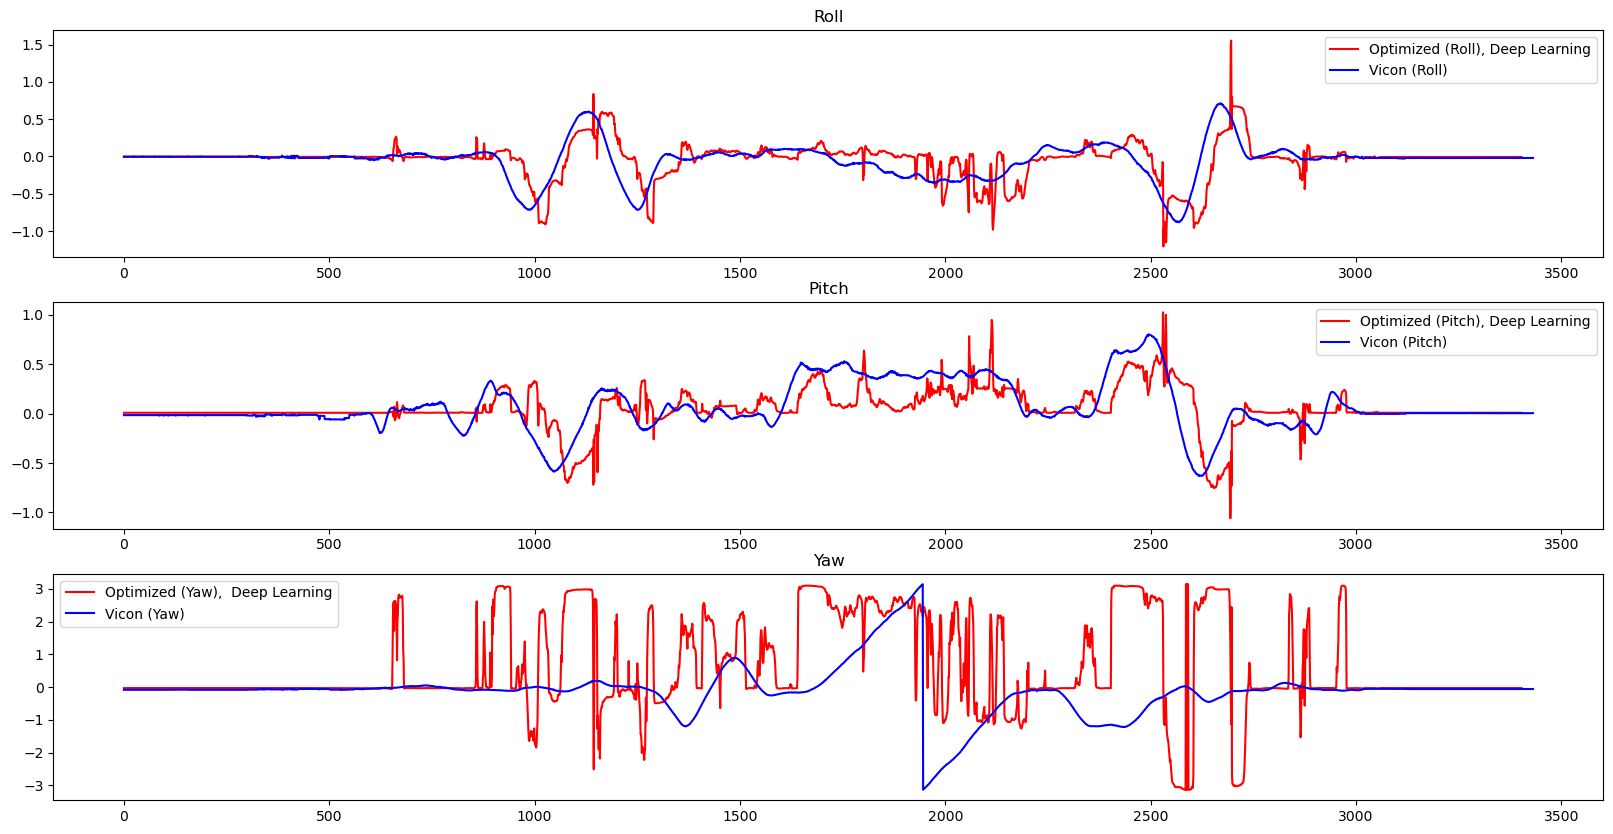
\includegraphics[width=1.0\textwidth]{images/dataset_3.png}}
\caption{Orientation Estimation for training dataset 3}
\label{fig:dataset_3}
\end{figure*}

\begin{figure*}[htbp]
  \centerline{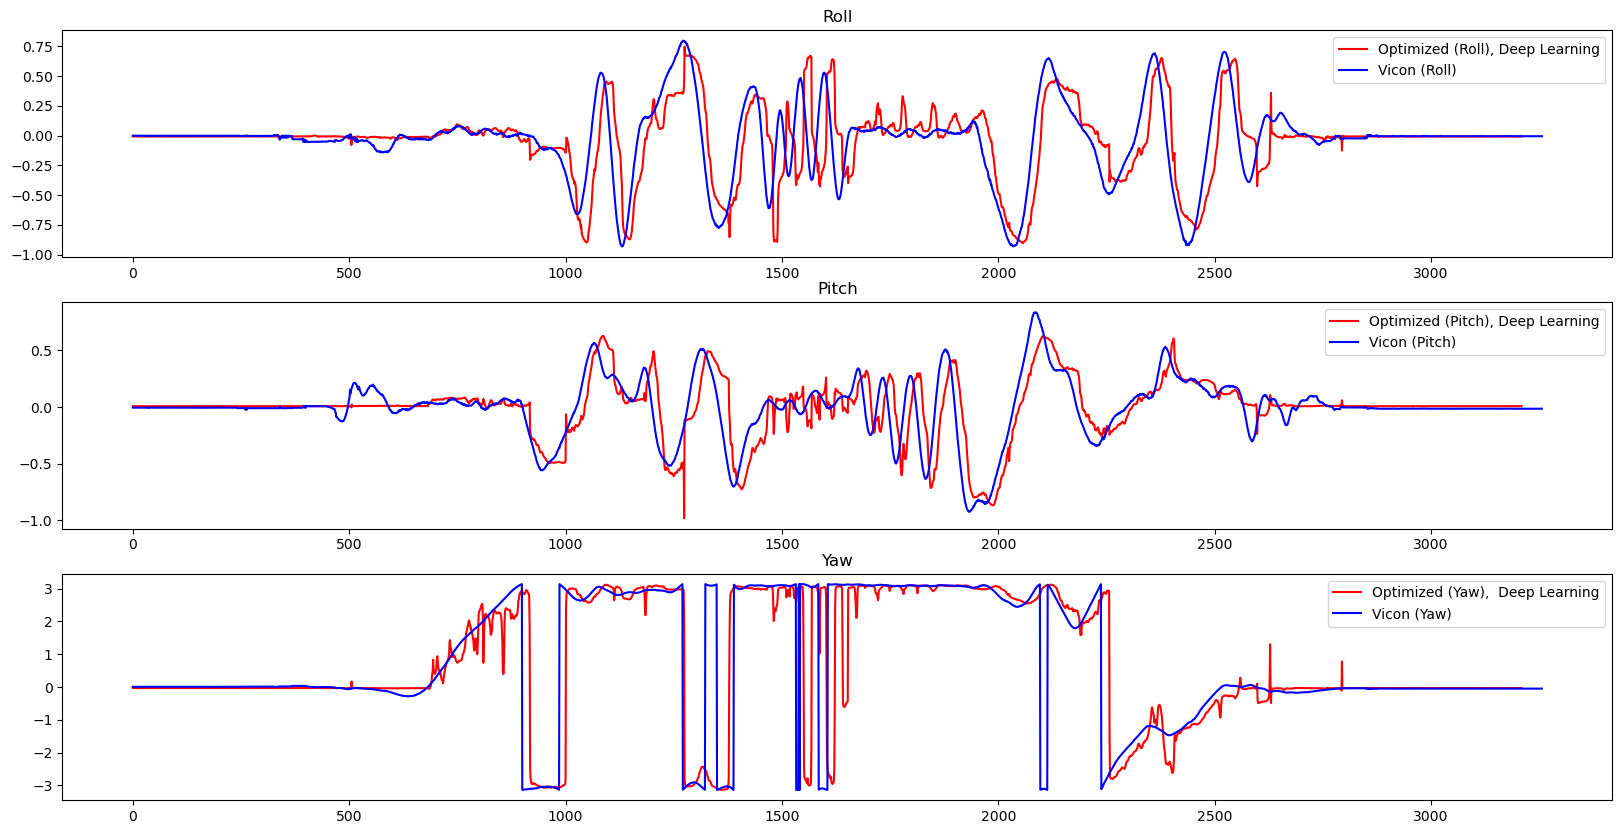
\includegraphics[width=1.0\textwidth]{images/dataset_5.png}}
\caption{Orientation Estimation for testing dataset 5}
\label{fig:dataset_5}
\end{figure*}

\section{Conclusion and Future Work}

This study has presented an innovative approach to 3D orientation tracking using a Neural Network methodology, leveraging IMU data to estimate the orientation of a rotating body. By formulating the problem as a minimization task and developing a custom loss function, we have demonstrated the potential of Neural Networks in orientation estimation tasks.

\subsection{Conclusion}
The Neural Network method, with its current reliance on future data and failure to capture sudden jumps (discontinuities) in the yaw angles, stands out only for its little reliance on parameter tuning but falls short on more accurate detection of discontinuities in the input data. However, with more datasets to train on, the Neural Network could potentially outperform the EKF methods in terms of robustness and accuracy, offering a promising alternative for 3D orientation tracking.

\subsection{Future Work}
Looking ahead, the potential for enhancing this Neural Network approach to suit real-time applications is an exciting
avenue for research. By investigating strategies to reduce reliance on future trajectory data, perhaps through the
incorporation of predictive models or real-time adaptive algorithms, it could be modified to offer its robustness in a real-time context. This could involve exploring iterative refinement techniques that allow for incremental updates to the orientation estimates as new data becomes available.

In conclusion, this work lays the groundwork for future innovations, highlighting the strengths and limitations of current methods while pointing towards potential improvements. The goal remains to develop an algorithm that combines the robustness of the Neural Network with the real-time capabilities of classical approaches like EKF, ensuring accurate, reliable, and efficient orientation tracking suitable for a wide array of applications.

\clearpage

\begin{thebibliography}{00}
\bibitem{b4} J. Solà, ``Quaternion kinematics for the error-state Kalman filter,'' [October 2017].
\bibitem{b7} A. Bani Younes and D. Mortari, ``Derivation of All Attitude Error Governing Equations for Attitude Filtering and Control,'' \textit{San Diego State University}, USA.
\bibitem{b6} Y-B. Jia, ``Quaternions,'' \textit{Com S 477/577 Notes}, December 2022.
\bibitem{b1} M. Kok, J. D. Hol, and T. B. Schön, ``Using Inertial Sensors for Position and Orientation Estimation,'' \textit{Delft University of Technology}, the Netherlands.
\bibitem{b2} Q. Yuan, E. Asadi, Q. Lu, G. Yang, and I-Ming Chen, ``Uncertainty Based IMU Orientation Tracking Algorithm for Dynamic Motions,'' \textit{IEEE Transactions}.
\bibitem{b3} B. Graf, ``Quaternions And Dynamics,'' \textit{EPFL}, February 2007.
\bibitem{b5} A. M. Sabatini, ``Quaternion-Based Extended Kalman Filter for Determining Orientation by Inertial and Magnetic Sensing,'' \textit{IEEE Transactions}.
\bibitem{b8} P. Wang, Z. Wang, and Q. Zhu, ``Attitude Estimation Based on Modified Two-stage EKF,'' \textit{Beijing University of Technology}, Beijing, China.
\bibitem{b9} F. M. Mirzaei and S. I. Roumeliotis, ``A Kalman Filter-Based Algorithm for IMU-Camera Calibration: Observability Analysis and Performance Evaluation,'' \textit{IEEE Transactions on Robotics}, vol. 24, no. 5, October 2008.
\end{thebibliography}
\vspace{12pt}

\end{document}
